\documentclass[aspectratio=169]{beamer}
\usetheme{Madrid}
\usecolortheme{beaver}
\usepackage[utf8]{inputenc}
\usepackage[T1]{fontenc}
\usepackage{tikz}
\usepackage{amssymb}
\usepackage{graphicx}
\setbeamertemplate{navigation symbols}{}
\setbeamercolor{title}{fg=white,bg=cyan!60!black}
\setbeamercolor{frametitle}{fg=white,bg=cyan!50!black}
\setbeamercolor{block title}{bg=cyan!15,fg=black}
\setbeamercolor{block body}{bg=cyan!5,fg=black}

\title{Block Arcade 4 — Variables}
\subtitle{BOSS: Score \& Lives HUD}
\author{ByteForge --- Grade 7 --- Game Maker}
\date{}

\begin{document}

\begin{frame}
    \titlepage
\end{frame}

\begin{frame}{BOSS — a real two-stat HUD}
    \Large
    Score AND lives, shown together, is genuinely what almost every simple arcade game's display actually is.

    \begin{center}
    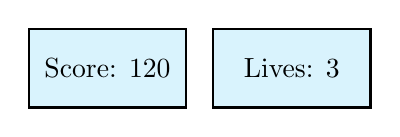
\begin{tikzpicture}[scale=0.9]

        \node[draw, thick, fill=cyan!15, minimum width=2cm, minimum height=1cm] at (0,0) {Score: 120};
        \node[draw, thick, fill=cyan!15, minimum width=2cm, minimum height=1cm] at (2.6,0) {Lives: 3};
    \end{tikzpicture}
    \end{center}
\end{frame}

\begin{frame}{Your Turn}
    \Large
    Open the student map, find \textbf{Block Arcade 4 — Variables}, and complete
    the \textbf{BOSS} challenge --- everything you just saw, they now do themselves.
\end{frame}

\end{document}
